\documentclass[a4 paper, 12pt]{article}
\usepackage[brazilian]{babel}
\usepackage[utf8]{inputenc}
\usepackage[T1]{fontenc}
\usepackage{minted}
\usepackage{anysize}
\usepackage{graphicx}
\marginsize{3cm}{3cm}{2cm}{2cm}
\usemintedstyle{tango}
\newminted{cpp}{linenos, mathescape, frame=topline, numberblanklines=false}
\newmint{cpp}{frame=single}
\usepackage{amsfonts}
\usepackage{amssymb}
\usepackage{amsmath}
\usepackage{algorithmic}
\usepackage[brazilian]{algorithm}
\renewcommand{\algorithmicrequire}{\textbf{Entrada:}}
\renewcommand{\algorithmicensure}{\textbf{Saída:}}
\renewcommand{\algorithmicend}{\textbf{fim}}
\renewcommand{\algorithmicif}{\textbf{se}}
\renewcommand{\algorithmicthen}{\textbf{então}}
\renewcommand{\algorithmicelse}{\textbf{else}}
\renewcommand{\algorithmicelsif}{\algorithmicelse\ \algorithmicif}
\renewcommand{\algorithmicendif}{\algorithmicend\ \algorithmicif}
\renewcommand{\algorithmicfor}{\textbf{para}}
\renewcommand{\algorithmicforall}{\textbf{para todos}}
\renewcommand{\algorithmicdo}{\textbf{faça}}
\renewcommand{\algorithmicendfor}{\algorithmicend}
\renewcommand{\algorithmicwhile}{\textbf{enquanto}}
\renewcommand{\algorithmicendwhile}{\algorithmicend}
\renewcommand{\algorithmicloop}{\textbf{loop}}
\renewcommand{\algorithmicendloop}{\algorithmicend\ \algorithmicloop}
\renewcommand{\algorithmicrepeat}{\textbf{repita}}
\renewcommand{\algorithmicuntil}{\textbf{enquanto}}
\renewcommand{\algorithmicprint}{\textbf{imprima}}
\renewcommand{\algorithmicreturn}{\textbf{retorne}}
\renewcommand{\algorithmictrue}{\textbf{verdadeiro}}
\renewcommand{\algorithmicfalse}{\textbf{falso}}


\renewcommand{\theFancyVerbLine}{
  \sffamily\textcolor[rgb]{0.5,0.5,0.5}{\scriptsize\arabic{FancyVerbLine}}}

\def\linha#1{
  \hbox to \hsize{
      \vbox{\centering #1}}
      \vspace{4mm}}

\begin{document}
\begin{titlepage}
\thispagestyle{empty}
\linha{\Huge \textbf {Universidade de São Paulo}}
\vspace{40mm}

%TÌtulo
\linha{\large PCS5730: Projeto e Técnicas de Construção de
  Compiladores\\}
\vspace{10mm}
\linha{\LARGE \textbf{\emph{There and back again}:\\Convertendo
    aut\^omatos para gram\'aticas}}
\vspace{50mm}
\linha{\large \textbf{Lucas Virgili}}

\vspace{50mm}
\linha{\large 1º Semestre de 2014}


\end{titlepage}
\tableofcontents

\vspace{4cm}
\section{Resumo}
Neste trabalho, propomos o desenvolvimento de um conjunto de
ferramentas que ser\'a usado para obter uma gram\'atica equivalente a
um aut\^omato, representado em forma de matriz.
\newpage
\section{Introdu\c c\~ao}
\'E bastante simples, a partir de uma gram\'atica livre de contexto
(as gram\'aticas do tipo 2 na hierarquia de Chomsky\cite{chomsky1956})
definida em nota\c c\~ao de Wirth, por exemplo, obter-se um aut\^omato
que reconhece uma senten\c ca escrita na gram\'atica como correta ou
incorreta\cite{parsingbook}.

N\~ao s\'o, Kleene\cite{kleene1956} mostrou a equival\^encia entre as
linguagens aceitas por aut\^omatos finitos e express\~oes
regulares. N\~ao s\'o, uma linguagem aceita por um aut\^omato finito
n\~ao deterministico pode ser representada por uma express\~ao
regular.

Assim, \'e poss\'ivel, pelo menos teoricamente, obter-se a partir de
um aut\^omato uma express\~ao regular equivalente, ou seja, que aceite
as mesmas senten\c cas corretas.

Tamb\'em sabemos que as linguagens geradas pelas gram\'aticas do tipo
3 na hierarquia de Chomsky definem as express\~oes regulares. Logo, a
partir de uma express\~ao regular podemos criar uma gram\'atica que a
gere. Claro que n\~ao necessariamente a melhor gram\'atica, mas uma
equivalente.

O objetivo deste trabalho foi propor um conjunto de ferramentas que,
dado um aut\^omato, gera uma gram\'atica equivalente a ele.


\section{Express\~oes regulares,  aut\^omatos e gram\'aticas}
\subsection{De aut\^omatos para express\~oes regulares}
Diversos m\'etodos existem para obter-se uma express\~ao regular
equivalente a um aut\^omato finito determin\'istico\cite{review1,
  review2}.

Infelizmente, o problema de se obter uma express\~ao regular m\'inima
\'e tanto PESPA\c CO-completo como NP-completo\cite{npcomplete}.

De forma geral, o tamanho da express\~ao est\'a relacionado \`a ordem
na qual os estados do aut\^omato s\~ao examinados. Logo, heur\'isticas
s\~ao utilizadas para obter-se uma express\~ao de tamanho aceit\'avel
em tempo e espa\c co razo\'aveis.

\subsubsection{Obtendo a express\~ao regular - M\'etodo baseado no fecho de Kleene}
Sejam $\{q_1, q_2, \ldots, q_k\}$ os estados do aut\^omato.

A ideia \'e usar um tipo de ``indu\c c\~ao'': seja $R_{i,j}^k$
a express\~ao regular para as entradas indo do estado $i$ ao estado
$j$, usando somente os $k$ primeiros estados do aut\^omato.

Para cada par $i, j$, suponha que $R_{i,j}$ represente a express\~ao
de $q_i$ at\'e $q_j$, mas sem usar o estado $q_k$. Agora, se pudermos
usar o estado $q_k$, podemos montar o novo $R$:
\begin{equation}
  \label{eq:1}
  R_{i,j}^{k} = R_{i,j}^{k-1} + R_{i,k}^{k-1} . R_{k,k}^{k-1*}. R_{k,j}^{k-1}
\end{equation}

Isso quer dizer que, para irmos de $i$ a $j$, podemos usar o que j\'a
sab\'iamos ou ir de $i$ at\'e o estado $k$, ficar em \emph{loop} em
$k$ e depois irmos de $k$ at\'e o estado $j$.
\newpage
O algoritmo, em ``pseudo python'':
\begin{minted}[mathescape, linenos=true, frame=lines]{python}
# Automato Sigma:
# n estados
# R matriz

# Inicializacao:
for i in range(1, n):
    for j in range(1, n):
        if i == j:
            R[i][j][0] = epsilon
        else:
            R[i][j][0] = nada
        for terminal in Sigma:
            if transicao(i, terminal, j):
                R[i][j][0] = R[i][j][0] + terminal

# Inducao
for k in range(1, n):
    for i in range(1, n):
        for j in range(1, n):
            R[i][j][k] = R[i][j][k-1] + R[i][k][k-1]
            . estrela_kleene(R[k][k][k-1]) . R[k][j][k-1]

# Regex
inicio = find_inicio(Sigma)
for i in range(1, n):
    if is_final(i):
        regex = regex + R[inicio][i][n]
\end{minted}

Esse algoritmo \'e claramente exponencial, tanto em espa\c c\o quanto
tempo. Contudo, ele demonstra a possibilidade ``pr\'atica'' da
convers\~ao.

\subsubsection{Obtendo a express\~ao regular - \emph{State elimination}}
An\'alises experimentais feitas durante esse trabalho mostraram que a
heur\'istica conhecima como \emph{state elimination}\cite{sr} gera express\~oes
regulares bastante pequenas em tempo aceit\'avel quando comparada com
diversas outras heur\'isticas propostas em \cite{heu}. Portanto ela foi
utilizada na nossa ferramenta.

O algoritmo de remo\c c\~ao de estado est\'a descrito a
seguir. Primeiro precisamos normalizar o aut\^omato, isto \'e, o
estado inicial n\~ao tem transi\c c\~oes para ele, h\'a apenas um
estado final e este estado n\~ao tem transi\c c\~oes saindo
dele. \'E trivial obter um aut\^omato normalizado a partir de um n\~ao
normalizado, basta adicionar dois estados ``falsos'' representando os
estados iniciais e finais e adicionar as transi\c c\~oes em vazio
adequadas.

Seja $Q$ o conjunto de estados do aut\^omato, $i$ o estado inicial e
$f$ o final. Tamb\'em denotamos por $\delta{q,a}$ o conjunto $\{p \in
Q | (q, a, p) \in \delta\}$, onde $\delta$ s\~ao as transi\c c\~oes,
$a$ \'e um s\'imbolo e $q\in Q$.

\begin{enumerate}
\item \textbf{Normaliza\c c\~ao}
\item \textbf{Elimina\c c\~ao de estado}
  \begin{enumerate}
  \item Se $Q=\{i,f\}$, a express\~ao procurada \'e $\alpha_{if}$ e o
    algoritmo termina. Caso contr\'ario v\'a para o pr\'oximo passo.
  \item Escolha um $q \in Q \backslash\{i,f\}$ e elime $q$ do aut\^omato, que
    passa a ter $Q \backslash \{q\}$ como conjunto de estados. Para cada estado
    $q_1, q_2$ nesse novo conjunto de estados fa\c ca:
    \begin{equation*}
      \delta'(q_1, q_2)=\alpha_{q1q2} + \alpha_{q1q}\alpha_{qq}*\alpha_{qq2}
    \end{equation*}
    Em seguida, retorne para o passo (a).
  \end{enumerate}
\end{enumerate}


\section{Ferramenta para obter a gram\'atica a partir de um
  aut\^omato}
Neste trabalho, desenvolemos duas ferramentas: a primeira, dada uma
matriz representando um aut\^omato, computa a representa\c c\~ao do
aut\^omato em express\~ao regular; a segunda converte uma express\~ao
regular em uma gram\'atica na nota\c c\~ao escolhida pelo
usu\'ario. Logo, utilizando as duas ferramentas em um
\emph{pipeline}, obtemos uma gram\'atica equivalente ao aut\^omato. A
figura \ref{fig:1} representa o processo.

\begin{figure}[H]
  \centering
  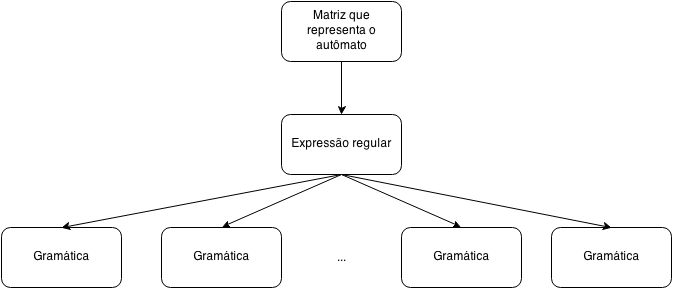
\includegraphics[width=0.8\textwidth]{estruturabranco.png}
  \caption{Oten\c c\~ao de gram\'aticas a partir do aut\^omato}
  \label{fig:1}
\end{figure}

\subsection{Do aut\^omato para a express\~ao regular}
O programa ``aut2regex.py'' recebe como par\^ametro um arquivo que
representa um aut\^omato e imprime uma express\~ao regular equivalente
ao aut\^omato.

O arquivo de entrada deve seguir o seguinte formato:
\begin{itemize}
\item ``\#'' \'e um coment\'ario
\item ``@DFA'' ou ``@NFA'' declara um novo aut\^omato e o seu
  tipo. Deve ser seguido pela lista de estados finais
\item Se for um NFA, pode haver um ``*'' seguido da lista de estados
  iniciais
\item Um ``\$'' opcional seguido da lista de s\'imbolos do alfabeto
\item A lista das transi\c c\~oes, que deve ser da seguinte forma:
  \begin{itemize}
  \item ``estado'' ``s\'imbolo'' ``novo estado''
  \end{itemize}
\item Uma transi\c c\~ao em vazio \'e denotada por ``@epsilon'' no
  caso de um NFA
\end{itemize}

Por exemplo, o aut\^omato representado na figura \ref{fig:2} tem o seguinte
arquivo de entrada:
\begin{figure}[H]
  \centering
  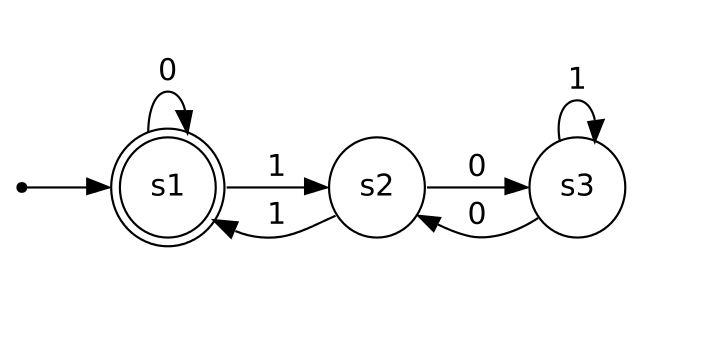
\includegraphics[width=0.5\pdfpagewidth]{output2.png}
  \caption{Aut\^omato exemplo}
  \label{fig:2}
\end{figure}

\begin{verbatim}
@DFA 0
0 1 1
0 0 0
1 1 0
1 0 2
2 1 2
2 0 1

\end{verbatim}

O programa tamb\'em pode ser usado sozinho para gerar express\~oes
regulares equivalentes.

\subsection{Da express\~ao para a gram\'atica}
Usando uma pilha e analisando a express\~ao \'e simples obter uma
gram\'atica equivalente em nota\c c\~ao de Wirth\footnote{A \'unica
  que eu tive tempo de implementar.}.

O programa ``regex2grammar.py'' converte uma express\~ao regular
passada como par\^ametro para uma gram\'atica e a imprime na sa\'ida
padr\~ao.

\subsection{A uni\~ao dos dois}
Seguindo a filosofia do UNIX, as duas ferramentas acima podem ser
unidas atrav\'es de um pipe e, a partir do arquivo que representa o
aut\^omato, imprimir a gram\'atica equivalente:
\begin{minted}[frame=lines]{bash}
python aut2regex.py arquivo_do_automato | python regex2grammar.py
\end{minted}

\section{Conclus\~ao}

\newpage
\begin{thebibliography}{99}

\bibitem{chomsky1956}
  Noam Chomsky,
  \emph{Three models for the description of language},
  IRE Transactions on Information Theory,
  (2): 113-24,
  1956

\bibitem{parsingbook}
  Dick Grune and Ceriel J. H. Jacobs,
  \emph{Parsing Techniques: A Practical Guide},
  Springer,
  2007

\bibitem{kleene1956}
  S. C. Kleene,
  \emph{Representation of events in nerve nets and finite automata},
  Automata Studies,
  3-41,
  Princeton University,
  1956

\bibitem{review1}
  K. Ellul, B. Krawetz, J. Shallit e M. Wang,
  \emph{Regular expressions: New results and open problems},
  J. Aut., Lang. and Combin.,
  10(4): 407-37,
  2005

\bibitem{review2}
  H. Gruber and M. Holzer,
  \emph{Provably shorter regular expressions from deterministic finite
  automata},
Proceedings of the 12th International Conference on Implementation and
Application of Automata,
(5462): 188-97,
Springer,
2008

\bibitem{npcomplete}
  T. Jiang and B. Ravikumar,
  \emph{Minimal NFA problems are hard}
  SIAM Journal of Computation,
  1117-41,
  1993

\bibitem{sr}
  J. A. Brzozowsk and E. J. McCluskey Jr.,
  \emph{Signal flow graph techniques for sequential circuit state
    diagrams},
  IEEE Trans. on Electronic Computers,
  EC-12(2): 67-76,
  1963

\bibitem{heu}
  Nelma Moreira, Davide Nabais e Rog\'erio Reis,
  \emph{State Elimination Ordering Strategies: Some Experimental
    Results},
  12th International Workshop on Descriptional Complexity of Formal
  systems,
  139-48,
  2010
\end{thebibliography}

\end{document}